\documentclass{exam}
\usepackage[utf8]{inputenc}
\usepackage{lmodern}
\usepackage{microtype}

% \usepackage[parfill]{parskip}
\usepackage[dvipsnames]{xcolor}
\usepackage{amsmath}
\usepackage{amsfonts}
\usepackage{amsthm}
\usepackage{siunitx}
\DeclareSIUnit\year{yr}
\DeclareSIUnit\foot{ft}
\DeclareSIUnit\litre{\liter}

\usepackage{skull}

\usepackage{pgfplots}
\usepgfplotslibrary{polar}
\pgfplotsset{compat=1.11}
\usepgfplotslibrary{statistics}
\usepackage{graphicx}
\usepackage{sidecap}
\sidecaptionvpos{figure}{c}
\usepackage{float}
\usepackage{gensymb}
\usepackage{tkz-euclide}
\usetkzobj{all}
\usepackage{commath}
\usepackage{hyperref}
\usepackage{enumitem}
\usepackage{wasysym}
\usepackage{multicol}
\usepackage{mathtools}
\usepackage{tcolorbox}
\usepackage{tabularx}
\usepackage[version=4]{mhchem}
\usepackage{changepage}
\usepackage{listings}
\lstset{basicstyle=\ttfamily\linespread{0.8}\small}

\renewcommand*{\thefootnote}{\fnsymbol{footnote}}

\newtheorem*{thm}{Theorem}
\newtheorem*{iden}{Identity}
\newtheorem*{lemma}{Lemma}
\newtheorem{obs}{Observation}
\theoremstyle{definition}
\newtheorem*{defn}{Definition}
\newtheorem*{ex}{Example}
\newtheorem{con}{Construction}
\newtheorem*{alg}{Algorithm}

\newtheoremstyle{break}
  {\topsep}{\topsep}%
  {\itshape}{}%
  {\bfseries}{}%
  {\newline}{}%
\theoremstyle{break}
\newtheorem*{bthm}{Theorem}

% russian integral
\usepackage{scalerel}
\DeclareMathOperator*{\rint}{\scalerel*{\rotatebox{17}{$\!\int\!$}}{\int}}

% \DeclareMathOperator*{\rint}{\int}

\pgfplotsset{vasymptote/.style={
    before end axis/.append code={
        \draw[densely dashed] ({rel axis cs:0,0} -| {axis cs:#1,0})
        -- ({rel axis cs:0,1} -| {axis cs:#1,0});
    }
}}

% \pointsinrightmargin
\boxedpoints
\pointname{}

\newcommand{\questioA}{\question[\texttt{\textbf{\color{Cerulean} A}}]}
\newcommand{\questioM}{\question[\texttt{\textbf{\color{PineGreen} M}}]}
\newcommand{\questioE}{\question[\texttt{\textbf{\color{WildStrawberry} E}}]}
\newcommand{\questioS}{\question[\texttt{\textbf{\color{Goldenrod} S}}]}
\newcommand{\questioO}{\question[\texttt{\textbf{\color{BurntOrange} O}}]}

\newcommand{\parA}{\part[\texttt{\textbf{\color{Cerulean} A}}]}
\newcommand{\parM}{\part[\texttt{\textbf{\color{PineGreen} M}}]}
\newcommand{\parE}{\part[\texttt{\textbf{\color{WildStrawberry} E}}]}
\newcommand{\parS}{\part[\texttt{\textbf{\color{Goldenrod} S}}]}
\newcommand{\parO}{\part[\texttt{\textbf{\color{BurntOrange} O}}]}

\newcommand{\subparA}{\subpart[\texttt{\textbf{\color{Cerulean} A}}]}
\newcommand{\subparM}{\subpart[\texttt{\textbf{\color{PineGreen} M}}]}
\newcommand{\subparE}{\subpart[\texttt{\textbf{\color{WildStrawberry} E}}]}
\newcommand{\subparS}{\subpart[\texttt{\textbf{\color{Goldenrod} S}}]}
\newcommand{\subparO}{\subpart[\texttt{\textbf{\color{BurntOrange} O}}]}

\newcommand{\mainHeader}[2]{\section*{NCEA Level 2 Mathematics\\#1. #2}}
\newcommand{\mainHeaderHw}[2]{\section*{NCEA Level 2 Mathematics (Homework)\\#1. #2}}
\newcommand{\seealso}[1]{\begin{center}\emph{See also #1.}\end{center}}
\newcommand{\drills}[1]{\begin{center}\emph{Drill problems: #1.}\end{center}}
\newcommand{\basedon}[1]{\begin{center}\emph{Notes largely based on #1.}\end{center}}

\begin{document}

\section*{NCEA Level 3 Calculus\\Revision: Functions}
Before we look at calculus proper, we need to revise a few things from our previous studies. Arguably, the most fundamental
concept from L2 is that of a function, together with its graph.

\begin{defn}[Function]
  A \textbf{function} is a relationship between two sets of things, called the \textit{range} and the \textit{domain}, such that
  everything in the range is related to exactly one thing in the domain. If $ f $ is a function which maps the value $ x $
  to the value $ y $, we write $ f : x \mapsto y $, or $ f(x) = y $. If $ f $ has range $ X $ and domain $ Y $, we write $ f : X \to Y $.

  Two functions $ f $ and $ g $ are called equal \emph{if and only if} the ranges of the two functions are the same \emph{and} for every $ x $ in that
  range, $ f(x) = g(x) $.
\end{defn}
You can think of a function as a rule: it could be given by a formula, or by a list of inputs and outputs, or in any other way that one wants.

\begin{defn}[Graph]
  If $ f $ is a function, then the set of all points $ (x,y) $ such that $ y = f(x) $ is called the \textbf{graph} of the function.
\end{defn}

\begin{exs}\leavevmode
  \begin{enumerate}
    \item The map which takes a number $ x $ and spits out $ x^2 $ is a function --- for every input, there is exactly one output. If
          we plot every point in the graph of this function, by plotting each input on the $ x-$axis and the corresponding output on
          the $ y-$axis, we obtain a parabola.
    \item The curve graphed below is \textit{not} the graph of a function, since for some inputs (like 1) the map has more than one output. We can check this
          by drawing vertical lines along the function, like that pictured: if a graph is a function, no vertical line can ever cross the curve
          more than once (this is the \textit{vertical-line test}).
          \begin{center}
            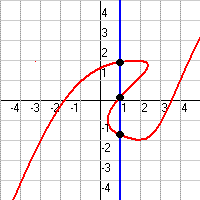
\includegraphics[width=0.3\textwidth]{linetest}
          \end{center}
    \item The map $ f : x \mapsto \sin x $ is a function (and so are all the other triangle ratios). We could also define it by `the
          function $ f $ such that $ f(x) = \sin x $'. This function $ f $ can only produce numbers between $1$ and $-1$; we say that
          its range is the interval from $ -1 $ to 1.
    \item On the other hand, to ensure that we obtain functions the inverse trigonometric maps must be restricted to certain inputs: to
          take a particular example, since there are infinitely many $ x $ so that $ \sin x = 1 $, there are infinitely many possibilities
          for the value of $ \arcsin x $. We will refrain from picking an explicit range for the inverse functions here and will generally
          just pick the most convenient at the time: it should be reasonably obvious from context.
    \item The map $ \iota : x \mapsto x $ is a function, called the \textit{identity function}.
    \item The map $ \ln x $ is a function, but it is only defined when $ x > 0 $: we say that its \textit{domain} is the positive real numbers.
    \item The following are some more non-examples of functions.
          \begin{center}
            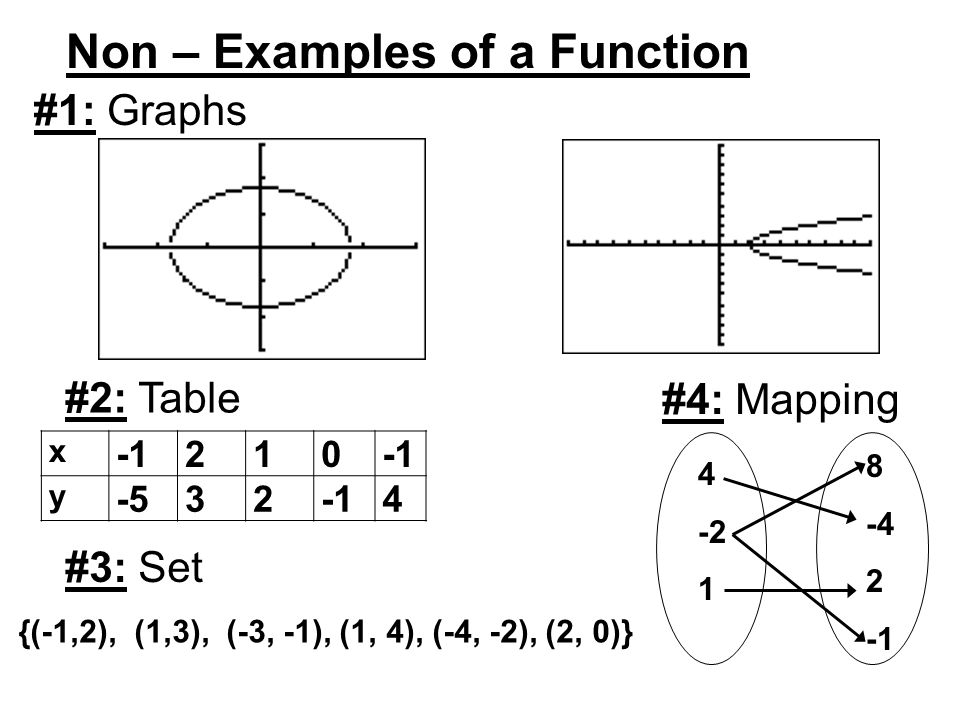
\includegraphics[width=0.5\textwidth]{notfunction}
          \end{center}
  \end{enumerate}
\end{exs}

\subsection*{Revision Questions}
\begin{questions}
  \question Which of the following are functions?
    \begin{parts}
      \part $ E(x) = 2^x $
      \part $ \phi : x \mapsto \frac{2}{x} $
      \part The thing which maps every person to their youngest sibling.
      \part The thing which sends every person to their youngest sibling that isn't themself.
      \part $ x \mapsto \lfloor x \rfloor $ (where $ \lfloor x \rfloor $ is the largest integer less than or equal to $ x $).
      \part The relation that sends every person to their age.
    \end{parts}
  \question I will define two functions, $ \varphi $ and $ \vartheta $, as follows:
            \begin{displaymath}
              \varphi(x) = 2x - 7, \qquad \vartheta(\zeta) = \frac{1}{7}(14\zeta - 49).
            \end{displaymath}
            Explain why these functions are equal.
  \question If $ f(x) = x^2 + x $, find:
    \begin{parts}
      \item $ f(1) $
      \item $ f(y) $
      \item $ f(x + h) $
    \end{parts}
  \question Find the distance between $ (-3, 4) $ and $ (2, 1) $.
  \question Three sides of a triangle are have lengths 8, 15, and 17.
    \begin{parts}
      \part Show that the triangle is right-angled.
      \part Find the other two angles.
    \end{parts}
  \question Factorise and solve $ x^2 - 3x + 2 = 0 $.
  \question How many \textbf{lines} are there through the point $ (2,3) $ and the origin? Give the equations of all such lines.
  \question Find the slope of the line $ 4x + 3y + 2 = 0 $.
  \question Find the solution to the following linear system:
            \begin{align*}
              2x + y &= 7\\
              3x - y &= 8
            \end{align*}
  \question How many (real) solutions does $ x^2 + 4x + 1 $ have?
  \question Draw $ \sin(x) $, $ \cos(x) $, $ \tan(x) $, $ \exp(x) $, and $ \ln(x) $.
  \question How many solutions does $ \cos (3\pi x + 1) = 2 $ have?
  \question How many solutions does $ \sin (3x) = \frac{1}{3} $ have?
\end{questions}

\end{document}
